\chapter{Grafs fortament connexos}

\index{graf fortament connex}

En un graf dirigit, les arestes només es poden recórrer en una
direcció, de manera que encara que el graf sigui connex, això no
garanteix que sempre hi hagi un camí dirigit entre dos nodes. Per aquest
motiu, definim un nou concepte més fort que el de connectivitat.

Un graf és \key{fortament connex} si hi ha un camí des de qualsevol
node a tots els altres nodes del graf. Per exemple, a la imatge
següent, el graf esquerre és fortament connex mentre que el graf dret
no.


\begin{center}
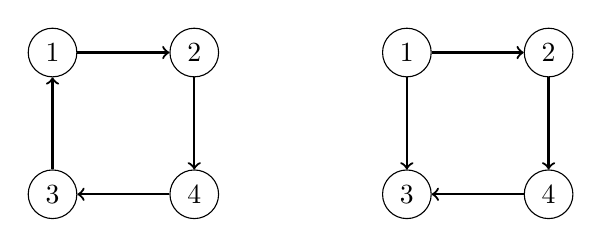
\begin{tikzpicture}[scale=0.9]
\node[draw, circle] (1) at (1,1) {$1$};
\node[draw, circle] (2) at (3,1) {$2$};
\node[draw, circle] (3) at (1,-1) {$3$};
\node[draw, circle] (4) at (3,-1) {$4$};

\path[draw,thick,->] (1) -- (2);
\path[draw,thick,->] (2) -- (4);
\path[draw,thick,->] (4) -- (3);
\path[draw,thick,->] (3) -- (1);

\node[draw, circle] (1b) at (6,1) {$1$};
\node[draw, circle] (2b) at (8,1) {$2$};
\node[draw, circle] (3b) at (6,-1) {$3$};
\node[draw, circle] (4b) at (8,-1) {$4$};

\path[draw,thick,->] (1b) -- (2b);
\path[draw,thick,->] (2b) -- (4b);
\path[draw,thick,->] (4b) -- (3b);
\path[draw,thick,->] (1b) -- (3b);
\end{tikzpicture}
\end{center}


El graf dret no és fortament connex perquè, per exemple, no hi ha cap
camí des del node 2 fins al node 1.

\index{components fortament connexes} \index{graf de components}

Les \key{components fortament connexes} d'un graf divideixen el graf
en parts fortament connexes tan grans com sigui possible. Les
components fortament connexes d'un graf formen un \key{graf de
  components}, que és un graf acíclic i dirigit que representa
l'estructura del graf original.

Per exemple, el graf
\begin{center}
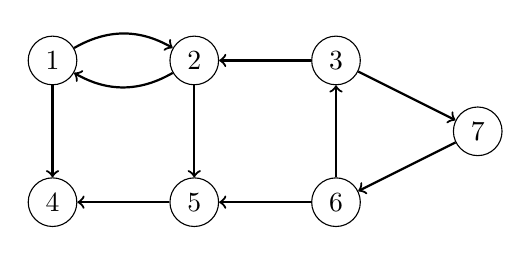
\begin{tikzpicture}[scale=0.9,label distance=-2mm]
\node[draw, circle] (1) at (-1,1) {$7$};
\node[draw, circle] (2) at (-3,2) {$3$};
\node[draw, circle] (4) at (-5,2) {$2$};
\node[draw, circle] (6) at (-7,2) {$1$};
\node[draw, circle] (3) at (-3,0) {$6$};
\node[draw, circle] (5) at (-5,0) {$5$};
\node[draw, circle] (7) at (-7,0) {$4$};

\path[draw,thick,->] (2) -- (1);
\path[draw,thick,->] (1) -- (3);
\path[draw,thick,->] (3) -- (2);
\path[draw,thick,->] (2) -- (4);
\path[draw,thick,->] (3) -- (5);
\path[draw,thick,->] (4) edge [bend left] (6);
\path[draw,thick,->] (6) edge [bend left] (4);
\path[draw,thick,->] (4) -- (5);
\path[draw,thick,->] (5) -- (7);
\path[draw,thick,->] (6) -- (7);
\end{tikzpicture}
\end{center}
té les següents components fortament connexes:
\begin{center}
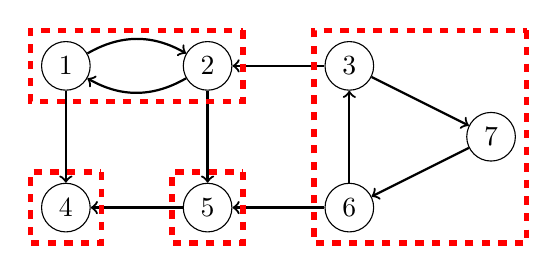
\begin{tikzpicture}[scale=0.9]
\node[draw, circle] (1) at (-1,1) {$7$};
\node[draw, circle] (2) at (-3,2) {$3$};
\node[draw, circle] (4) at (-5,2) {$2$};
\node[draw, circle] (6) at (-7,2) {$1$};
\node[draw, circle] (3) at (-3,0) {$6$};
\node[draw, circle] (5) at (-5,0) {$5$};
\node[draw, circle] (7) at (-7,0) {$4$};

\path[draw,thick,->] (2) -- (1);
\path[draw,thick,->] (1) -- (3);
\path[draw,thick,->] (3) -- (2);
\path[draw,thick,->] (2) -- (4);
\path[draw,thick,->] (3) -- (5);
\path[draw,thick,->] (4) edge [bend left] (6);
\path[draw,thick,->] (6) edge [bend left] (4);
\path[draw,thick,->] (4) -- (5);
\path[draw,thick,->] (5) -- (7);
\path[draw,thick,->] (6) -- (7);

\draw [red,thick,dashed,line width=2pt] (-0.5,2.5) rectangle (-3.5,-0.5);
\draw [red,thick,dashed,line width=2pt] (-4.5,2.5) rectangle (-7.5,1.5);
\draw [red,thick,dashed,line width=2pt] (-4.5,0.5) rectangle (-5.5,-0.5);
\draw [red,thick,dashed,line width=2pt] (-6.5,0.5) rectangle (-7.5,-0.5);
\end{tikzpicture}
\end{center}
El graf de components corresponent és el següent:
\begin{center}
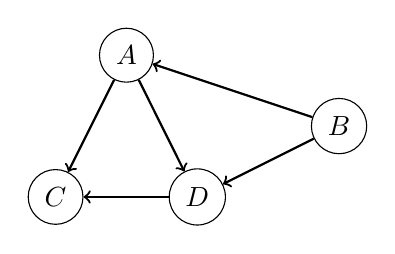
\begin{tikzpicture}[scale=0.9]
\node[draw, circle] (1) at (-3,1) {$B$};
\node[draw, circle] (2) at (-6,2) {$A$};
\node[draw, circle] (3) at (-5,0) {$D$};
\node[draw, circle] (4) at (-7,0) {$C$};

\path[draw,thick,->] (1) -- (2);
\path[draw,thick,->] (1) -- (3);
\path[draw,thick,->] (2) -- (3);
\path[draw,thick,->] (2) -- (4);
\path[draw,thick,->] (3) -- (4);
\end{tikzpicture}
\end{center}
Les components són $A=\{1,2\}$, $B=\{3,6,7\}$, $C=\{4\}$ i $D=\{5\}$.

Com que el graf de components és acíclic i dirigit, és més fàcil de
processar que el graf original. Com que el graf no conté cicles,
sempre podem construir una ordenació topològica i utilitzar tècniques
de programació dinàmica del capítol 16.

\section{Algorisme de Kosaraju}

\index{Algorisme de Kosaraju}

L'\key{algorisme de Kosaraju}\footnote{Segons \cite{aho83},
S. R. Kosaraju va inventar aquest algorisme l'any 1978 però no el va
publicar. El 1981, el mateix algorisme va ser redescobert i publicat
per M. Sharir \cite{sha81}.} és un mètode eficient per trobar les
components fortament connexes d'un graf dirigit. L'algorisme
realitza dues cerques en profunditat: la primera cerca construeix una
llista de nodes segons l'estructura del graf, i la segona cerca forma
les components fortament connectats.

\subsubsection{Cerca 1}

La primera fase de l'algorisme de Kosaraju construeix una llista de
nodes en l'ordre en el que apareixen en una cerca en
profunditat. L'algorisme itera pels nodes i comença una cerca en
profunditat per cada node no processat. Cada node s'afegeix a la llista
un cop s'ha processat.

En aquest exemple els nodes es processen en l'ordre següent:
\begin{center}
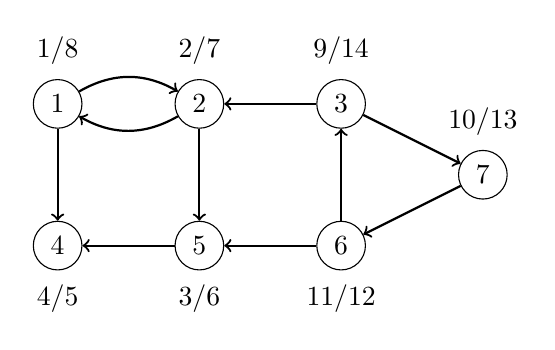
\begin{tikzpicture}[scale=0.9,label distance=-2mm]
\node[draw, circle] (1) at (-1,1) {$7$};
\node[draw, circle] (2) at (-3,2) {$3$};
\node[draw, circle] (4) at (-5,2) {$2$};
\node[draw, circle] (6) at (-7,2) {$1$};
\node[draw, circle] (3) at (-3,0) {$6$};
\node[draw, circle] (5) at (-5,0) {$5$};
\node[draw, circle] (7) at (-7,0) {$4$};

\node at (-7,2.75) {$1/8$};
\node at (-5,2.75) {$2/7$};
\node at (-3,2.75) {$9/14$};
\node at (-7,-0.75) {$4/5$};
\node at (-5,-0.75) {$3/6$};
\node at (-3,-0.75) {$11/12$};
\node at (-1,1.75) {$10/13$};

\path[draw,thick,->] (2) -- (1);
\path[draw,thick,->] (1) -- (3);
\path[draw,thick,->] (3) -- (2);
\path[draw,thick,->] (2) -- (4);
\path[draw,thick,->] (3) -- (5);
\path[draw,thick,->] (4) edge [bend left] (6);
\path[draw,thick,->] (6) edge [bend left] (4);
\path[draw,thick,->] (4) -- (5);
\path[draw,thick,->] (5) -- (7);
\path[draw,thick,->] (6) -- (7);
\end{tikzpicture}
\end{center}


Fem servir la notació $x/y$ per a indicar que el node s'ha començat a
processar en el pas $x$ i s'ha acabat de processar en el pas
$y$. La llista resultant és la següent:


\begin{tabular}{ll}
\\
node & pas de final de processament \\
\hline
4 & 5 \\
5 & 6 \\
2 & 7 \\
1 & 8 \\
6 & 12 \\
7 & 13 \\
3 & 14 \\
\\
\end{tabular}

\footnote{(N. del T.) La propietat clau d'aquesta llista és que si, es pot anar
de $u$ a $v$ però no és pot anar de $v$ a $u$, es té que $v$ apareix
abans que $u$ en la llista. Dit d'altra manera: la llista ordena els
nodes en \emph{ordre topològic invers} de les components fortament
connexes respectives en el graf de components.}

\subsubsection{Cerca 2}

En la segona fase de l'algorisme formem les components fortament
connexes del graf. En primer lloc, l'algorisme inverteix totes les
arestes del graf. Després d'invertir les arestes, el graf d'exemple és el següent:
\begin{center}
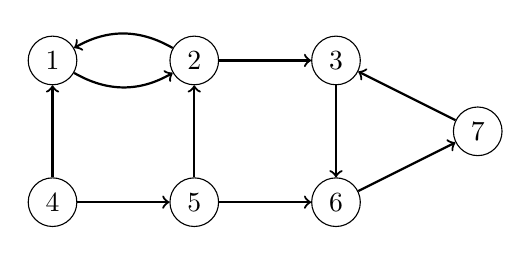
\begin{tikzpicture}[scale=0.9,label distance=-2mm]
\node[draw, circle] (1) at (-1,1) {$7$};
\node[draw, circle] (2) at (-3,2) {$3$};
\node[draw, circle] (4) at (-5,2) {$2$};
\node[draw, circle] (6) at (-7,2) {$1$};
\node[draw, circle] (3) at (-3,0) {$6$};
\node[draw, circle] (5) at (-5,0) {$5$};
\node[draw, circle] (7) at (-7,0) {$4$};

\path[draw,thick,<-] (2) -- (1);
\path[draw,thick,<-] (1) -- (3);
\path[draw,thick,<-] (3) -- (2);
\path[draw,thick,<-] (2) -- (4);
\path[draw,thick,<-] (3) -- (5);
\path[draw,thick,<-] (4) edge [bend left] (6);
\path[draw,thick,<-] (6) edge [bend left] (4);
\path[draw,thick,<-] (4) -- (5);
\path[draw,thick,<-] (5) -- (7);
\path[draw,thick,<-] (6) -- (7);
\end{tikzpicture}
\end{center}

Ara l'algorisme recorre en ordre \emph{invers} la llista de nodes
creats per la primera cerca. Per cada node que encara no pertany a cap
component, l'algorisme crea una nova component i inicia una cerca en
profunditat que afegeix tots els nodes nous trobats a la nova
component.

Al graf d'exemple, la primera component comença al node 3:


\begin{center}
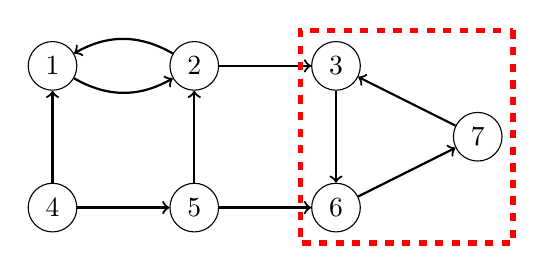
\begin{tikzpicture}[scale=0.9,label distance=-2mm]
\node[draw, circle] (1) at (-1,1) {$7$};
\node[draw, circle] (2) at (-3,2) {$3$};
\node[draw, circle] (4) at (-5,2) {$2$};
\node[draw, circle] (6) at (-7,2) {$1$};
\node[draw, circle] (3) at (-3,0) {$6$};
\node[draw, circle] (5) at (-5,0) {$5$};
\node[draw, circle] (7) at (-7,0) {$4$};

\path[draw,thick,<-] (2) -- (1);
\path[draw,thick,<-] (1) -- (3);
\path[draw,thick,<-] (3) -- (2);
\path[draw,thick,<-] (2) -- (4);
\path[draw,thick,<-] (3) -- (5);
\path[draw,thick,<-] (4) edge [bend left] (6);
\path[draw,thick,<-] (6) edge [bend left] (4);
\path[draw,thick,<-] (4) -- (5);
\path[draw,thick,<-] (5) -- (7);
\path[draw,thick,<-] (6) -- (7);

\draw [red,thick,dashed,line width=2pt] (-0.5,2.5) rectangle (-3.5,-0.5);
\end{tikzpicture}
\end{center}

Tingueu en compte que, com que totes les arestes estan invertides, no
es possible ``escapar-se'' a altres parts del graf. (N. del T.) Com
que tractem els nodes en ordre topològic de les components fortament
connexes, quan tractem una component sabem que ja hem acabat de
tractar totes aquelles altres components des de les quals es podia
arribar a la nostra en el graf original. Això garantitza que la segona
cerca no pot sortir de la component fortament connexa.

Els nodes següents a la llista són els nodes 7 i 6, però ja pertanyen
a una component, de manera que la nova component comença al node 1:

\begin{center}
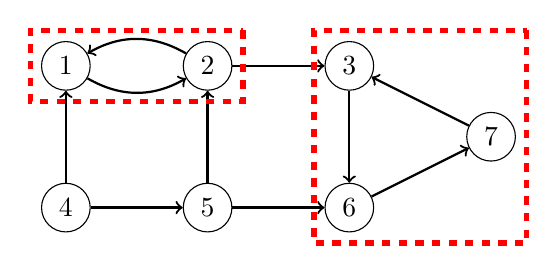
\begin{tikzpicture}[scale=0.9,label distance=-2mm]
\node[draw, circle] (1) at (-1,1) {$7$};
\node[draw, circle] (2) at (-3,2) {$3$};
\node[draw, circle] (4) at (-5,2) {$2$};
\node[draw, circle] (6) at (-7,2) {$1$};
\node[draw, circle] (3) at (-3,0) {$6$};
\node[draw, circle] (5) at (-5,0) {$5$};
\node[draw, circle] (7) at (-7,0) {$4$};

\path[draw,thick,<-] (2) -- (1);
\path[draw,thick,<-] (1) -- (3);
\path[draw,thick,<-] (3) -- (2);
\path[draw,thick,<-] (2) -- (4);
\path[draw,thick,<-] (3) -- (5);
\path[draw,thick,<-] (4) edge [bend left] (6);
\path[draw,thick,<-] (6) edge [bend left] (4);
\path[draw,thick,<-] (4) -- (5);
\path[draw,thick,<-] (5) -- (7);
\path[draw,thick,<-] (6) -- (7);

\draw [red,thick,dashed,line width=2pt] (-0.5,2.5) rectangle (-3.5,-0.5);
\draw [red,thick,dashed,line width=2pt] (-4.5,2.5) rectangle (-7.5,1.5);
%\draw [red,thick,dashed,line width=2pt] (-4.5,0.5) rectangle (-5.5,-0.5);
%\draw [red,thick,dashed,line width=2pt] (-6.5,0.5) rectangle (-7.5,-0.5);
\end{tikzpicture}
\end{center}

Finalment, l'algorisme processa els nodes 5 i 4 que creen les
components fortament connexes que falten:

\begin{center}
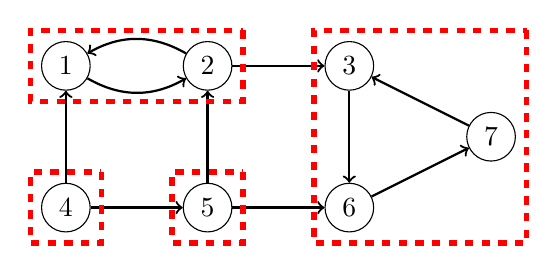
\begin{tikzpicture}[scale=0.9,label distance=-2mm]
\node[draw, circle] (1) at (-1,1) {$7$};
\node[draw, circle] (2) at (-3,2) {$3$};
\node[draw, circle] (4) at (-5,2) {$2$};
\node[draw, circle] (6) at (-7,2) {$1$};
\node[draw, circle] (3) at (-3,0) {$6$};
\node[draw, circle] (5) at (-5,0) {$5$};
\node[draw, circle] (7) at (-7,0) {$4$};

\path[draw,thick,<-] (2) -- (1);
\path[draw,thick,<-] (1) -- (3);
\path[draw,thick,<-] (3) -- (2);
\path[draw,thick,<-] (2) -- (4);
\path[draw,thick,<-] (3) -- (5);
\path[draw,thick,<-] (4) edge [bend left] (6);
\path[draw,thick,<-] (6) edge [bend left] (4);
\path[draw,thick,<-] (4) -- (5);
\path[draw,thick,<-] (5) -- (7);
\path[draw,thick,<-] (6) -- (7);

\draw [red,thick,dashed,line width=2pt] (-0.5,2.5) rectangle (-3.5,-0.5);
\draw [red,thick,dashed,line width=2pt] (-4.5,2.5) rectangle (-7.5,1.5);
\draw [red,thick,dashed,line width=2pt] (-4.5,0.5) rectangle (-5.5,-0.5);
\draw [red,thick,dashed,line width=2pt] (-6.5,0.5) rectangle (-7.5,-0.5);
\end{tikzpicture}
\end{center}


La complexitat temporal de l'algorisme és $O(n+m)$, perquè l'algorisme
realitza dues cerques en profunditat.

\section{Problema 2SAT}

\index{Problema 2SAT}

Els grafs fortament connexos també estan relacionats amb el problema
\key{2SAT}\footnote{L'algorisme que es presenta aquí es va introduir a
\cite{asp79}. També hi ha un altre algorisme de temps lineal conegut
\cite{eve75} que es basa en el retrocés (backtracking).}. En aquest
problema, se'ns dóna una fórmula lògica
\[
(a_1 \lor b_1) \land (a_2 \lor b_2) \land \cdots \land (a_m \lor b_m),
\]
on cada $a_i$ i $b_i$ és una variable lògica ($x_1,x_2,\ldots,x_n$) o
una negació d'una variable lògica ($\lnot x_1, \lnot x_2, \ldots,
\lnot x_n$ ). Els símbols ''$\land$'' i ''$\lor$'' denoten operadors
lògics ''AND'' i ''OR''. La nostra tasca és assignar un valor a cada
variable perquè la fórmula sigui certa, o bé afirmar que això no és
possible.

Per exemple, la fórmula
\[
L_1 = (x_2 \lor \lnot x_1) \land
      (\lnot x_1 \lor \lnot x_2) \land
      (x_1 \lor x_3) \land
      (\lnot x_2 \lor \lnot x_3) \land
      (x_1 \lor x_4)
\]
és certa quan les variables s'assignen de la següent manera:


\[
\begin{cases}
x_1 = \textrm{false} \\
x_2 = \textrm{false} \\
x_3 = \textrm{true} \\
x_4 = \textrm{true} \\
\end{cases}
\]


Tanmateix, la fórmula
\[
L_2 = (x_1 \lor x_2) \land
      (x_1 \lor \lnot x_2) \land
      (\lnot x_1 \lor x_3) \land
      (\lnot x_1 \lor \lnot x_3)
\]
sempre és falsa, independentment de com assignem els valors. El motiu
és que no podem triar un valor per a $x_1$ sense crear una
contradicció. Si $x_1$ és fals, tant $x_2$ com $\lnot x_2$ han de ser
certs, cosa que és impossible; i si $x_1$ és cert, tant $x_3$ com
$\lnot x_3$ han de ser certs, cosa que també és impossible.

El problema 2SAT es pot representar com un graf els nodes del qual es
corresponen amb variables $x_i$ i negacions $\lnot x_i$, i les arestes
determinen les connexions entre les variables.  Cada parell $(a_i \lor
b_i)$ genera dues arestes: $\lnot a_i \to b_i$ i $\lnot b_i \to
a_i$. Això vol dir que si $a_i$ no es certa, $b_i$ ha de ser certa, i
viceversa. \footnote{(N. del T.) És útil interpretar una aresta dirigida
$(x,y)$ com ``$x$ implica $y$'', i un camí dirigit com una cadena d'implicacions
lògiques.}

El graf de la fórmula $L_1$ és: \\
\begin{center}
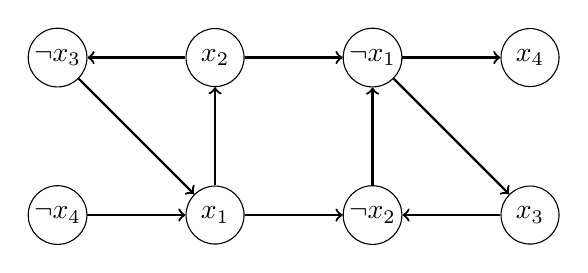
\begin{tikzpicture}[scale=1.0,minimum size=2pt]
\node[draw, circle, inner sep=1.3pt] (1) at (1,2) {$\lnot x_3$};
\node[draw, circle] (2) at (3,2) {$x_2$};
\node[draw, circle, inner sep=1.3pt] (3) at (1,0) {$\lnot x_4$};
\node[draw, circle] (4) at (3,0) {$x_1$};
\node[draw, circle, inner sep=1.3pt] (5) at (5,2) {$\lnot x_1$};
\node[draw, circle] (6) at (7,2) {$x_4$};
\node[draw, circle, inner sep=1.3pt] (7) at (5,0) {$\lnot x_2$};
\node[draw, circle] (8) at (7,0) {$x_3$};
 
\path[draw,thick,->] (1) -- (4);
\path[draw,thick,->] (4) -- (2);
\path[draw,thick,->] (2) -- (1);
\path[draw,thick,->] (3) -- (4);
\path[draw,thick,->] (2) -- (5);
\path[draw,thick,->] (4) -- (7);
\path[draw,thick,->] (5) -- (6);
\path[draw,thick,->] (5) -- (8);
\path[draw,thick,->] (8) -- (7);
\path[draw,thick,->] (7) -- (5);
\end{tikzpicture}
\end{center}
I el graf de la fórmula $L_2$ és: \\
\begin{center}
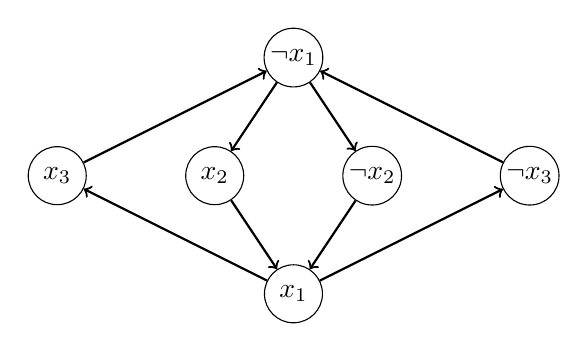
\begin{tikzpicture}[scale=1.0,minimum size=2pt]
\node[draw, circle] (1) at (1,2) {$x_3$};
\node[draw, circle] (2) at (3,2) {$x_2$};
\node[draw, circle, inner sep=1.3pt] (3) at (5,2) {$\lnot x_2$};
\node[draw, circle, inner sep=1.3pt] (4) at (7,2) {$\lnot x_3$};
\node[draw, circle, inner sep=1.3pt] (5) at (4,3.5) {$\lnot x_1$};
\node[draw, circle] (6) at (4,0.5) {$x_1$};

\path[draw,thick,->] (1) -- (5);
\path[draw,thick,->] (4) -- (5);
\path[draw,thick,->] (6) -- (1);
\path[draw,thick,->] (6) -- (4);
\path[draw,thick,->] (5) -- (2);
\path[draw,thick,->] (5) -- (3);
\path[draw,thick,->] (2) -- (6);
\path[draw,thick,->] (3) -- (6);
\end{tikzpicture}
\end{center}


L'estructura del graf ens indica si és possible assignar valors a les
variables de manera que la fórmula sigui certa. Resulta que això es
pot fer exactament quan no hi ha nodes $x_i$ i $\lnot x_i$ que
pertanyin a la mateixa component fortament connexa. Si existeixen
aquests nodes, aleshores el graf conté un camí de $x_i$ a $\lnot x_i$
i també un camí de $\lnot x_i$ a $x_i$, de manera que $x_i$ implica
$\lnot x_i$ i $\lnot x_i$ implica $x_i$, cosa que no és possible.

Al graf de la fórmula $L_1$ no hi ha nodes $x_i$ i $\lnot x_i$ que
pertanyin a la mateixa component fortament connexa, de manera que
existeix una solució. Al graf de la fórmula $L_2$ tots els nodes
pertanyen a la mateixa component fortament connexa, i no hi ha cap
solució.

Si existeix una solució, els valors de les variables es poden trobar
passant pels nodes del graf de components en un ordre topològic
invers. A cada pas, processem una component que no conté arestes que
condueixin a una component sense processar. Si no s'han assignat
valors a les variables de la component, busquem una assignació de
valors compatible, i si ja tenen valors, no els canviem. El procés
continua fins que a cada variable se li ha assignat un valor.

El graf de components per a la fórmula $L_1$ és el següent:
\begin{center}
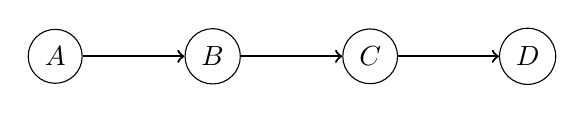
\begin{tikzpicture}[scale=1.0]
\node[draw, circle] (1) at (0,0) {$A$};
\node[draw, circle] (2) at (2,0) {$B$};
\node[draw, circle] (3) at (4,0) {$C$};
\node[draw, circle] (4) at (6,0) {$D$};

\path[draw,thick,->] (1) -- (2);
\path[draw,thick,->] (2) -- (3);
\path[draw,thick,->] (3) -- (4);
\end{tikzpicture}
\end{center}


Les components són $A = \{\lnot x_4\}$, $B = \{x_1, x_2, \lnot x_3\}$,
$C = \{\lnot x_1, \lnot x_2, x_3\}$ i $ D = \{x_4\}$. Quan construïm
la solució, primer processem la component $D$, i $x_4$ esdevé
cert. Després d'això, processem la component $C$ on $x_1$ i $x_2$
esdevenen falsos i $x_3$ esdevé cert. Totes les variables tenen valors
assignats, de manera que les components restants $A$ i $B$ no canvien
les variables.

Tingueu en compte que aquest mètode funciona perquè el graf té una
estructura especial: si hi ha camins des del node $x_i$ al node $x_j$
i des del node $x_j$ al node $\lnot x_j$, aleshores el node $x_i$ mai
no pot ser cert. El motiu es que també ha d'haver-hi un camí des del node
$\lnot x_j$ fins al node $\lnot x_i$, i tant $x_i$ com $x_j$ esdevenen
falsos.

\index{Problema 3SAT}

Un problema més difícil és el \key{problema 3SAT}, on cada part de la
fórmula és de la forma $(a_i \lor b_i \lor c_i)$, on $a_i, b_i$ i
$c_i$ són també variables lògiques o les seves negacions. Aquest
problema és NP-difícil, de manera que no es coneix cap algorisme
eficient que el resolgui.


